% TU Delft Beamer template
% Author: Maarten Abbink
% Delft University of Technology
% March 2014
% Version 2.0
% Based on original version 1.0 of Carl Schneider
\documentclass{beamer}
\usepackage[english]{babel}
\usepackage{calc}
\usepackage[absolute,overlay]{textpos}

\mode<presentation>{\usetheme{default} \usecolortheme{seahorse}}

\title[BEP]{Virtual Asssitant Web App\\ \small{Bachelor Thesis}}
%\subtitle
\institute[TU Delft]{Delft University of Technology}
\author{A. Hambenne\\
S. Jahanshahi}
\date{\today}

% Insert frame before each subsection (requires 2 latex runs)
\AtBeginSubsection[] {
	\begin{frame}<beamer>\frametitle{\titleSubsec}
		\tableofcontents[currentsection,currentsubsection]  % Generation of the Table of Contents
	\end{frame}
}	


% define a symbol which can be removed if you don't need it
\newcommand{\field}[1]{\mathbb{#1}}
\newcommand{\Zset}{\field{Z}}

\begin{document}

{
% remove the next line if you don't want a background image
\usebackgroundtemplate{
\includegraphics[width=\paperwidth,height=\paperheight]{images/background-titlepage.jpg}}%
\setbeamertemplate{footline}{\usebeamertemplate*{minimal footline}}
\frame{\titlepage}
}

{\setbeamertemplate{footline}{\usebeamertemplate*{minimal footline}}
% \begin{frame}\frametitle{\titleTOC}
% 	\tableofcontents
% \end{frame}
}



\begin{frame}\frametitle{Outline}
	\begin{itemize}
		\item What is our project about?
		\item Project Set-up
		\item Research \& Planning
		\item Technologies
		\item Design Architecture
		\item Features
		\item Metrics  \& Evaluation
		\item Demo
		\item Q\&A Session
	\end{itemize}
\end{frame}

% FEATURES

%OAUTH2
\begin{frame}
\frametitle{Features}
\framesubtitle{OAuth2 Authentication}
	\begin{itemize}
		\item Allowing users to authenticate themselves through accounts from other webservices
		\item Google Plus and Mendeley
		\item Use of existing Google Plus OAuth2 library
		\item Extended library for Mendeley
		\item Library can also be used for Facebook, Twitter, GitHub,...
	\end{itemize}
\end{frame}

%PROJECT
\begin{frame}
\frametitle{Features}
\framesubtitle{Projects}
	\begin{itemize}
		\item A project is a virtual entity that users can create and join
		\item Users who join get assigned a role by the inviting member
		\item Three roles for members available: Owner, Reviewer and Guest
		\item Predefined template vs. own template
		\item Documents uploadable only by owners and reviewers, downloadable by every member
		\item Projects can not be joined or searched by users without invitation
	\end{itemize}
\end{frame}

%DISCUSSION
\begin{frame}
\frametitle{Features}
\framesubtitle{Discussions}
	\begin{itemize}
		\item Discussions are linked to a project
		\item Multiple discussions can be held per project
		\item Discussions are visible and accessible to every member of the project
		\item The use of AngularJS allows for real-time comment rendering (chat-like)
		\item A discussion consists of one top-comment with zero or more sub-comments
	\end{itemize}
\end{frame}

%TASKS
\begin{frame}
\frametitle{Features}
\framesubtitle{Tasks}
	\begin{itemize}
		\item Tasks are exclusively linked to users
		\item Have a due date and a description
		\item Can be marked as Done and To-Do
		\item Can be deleted and redone
		\item Due dates do not show on Calendar
	\end{itemize}
\end{frame}

%MENDELEY LIBRARY SHARING
\begin{frame}
\frametitle{Features}
\framesubtitle{Mendeley Library Sharing}
	\begin{itemize}
		\item Users can link their Mendeley Library to the application
		\item Linking imports all the metadata as models into the application
		\item When a user wants to add a document to his/her Mendeley Library, the metadata gets posted through OAuth2 API
		\item Users can also sync their library again in case external changes were made
		\item Mendeley Library Sharing is a global feature
	\end{itemize}
\end{frame}

%FORM VALIDATION
\begin{frame}
\frametitle{Features}
\framesubtitle{Form Validation}
	\begin{itemize}
		\item A user must always have a valid session to access a page or perform an action
		\item Names and titles of users and projects are passed through a REGEX expression
	\end{itemize}
\end{frame}

%METRICS 1
\begin{frame}
\frametitle{Metrics \& Evaluation}
\framesubtitle{GitHub \& Code}
	\begin{figure}
		
\includegraphics[scale=0.3]{./images/github_stats.png}
		\caption{GitHub Statistics}
	\end{figure}
	\begin{itemize}
		\item Total lines of code: \textbf{5341} (including statically imported plugins)
		\item Total code coverage: \textbf{69\%} (excluding statically imported plugins and framework code)
	\end{itemize}
	\begin{figure}
		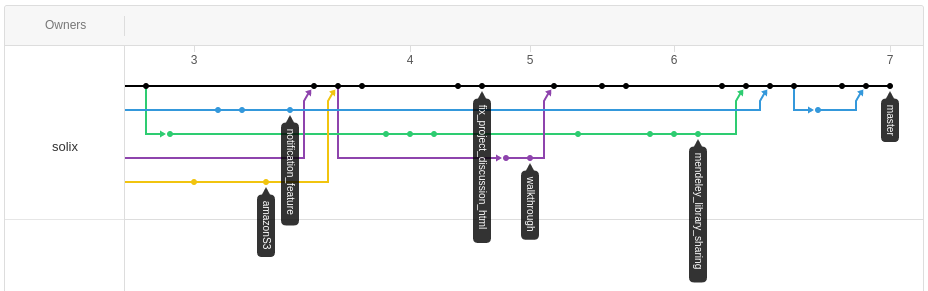
\includegraphics[scale=0.2]{./images/github_tree.png}
		\caption{GitHub Branching Tree}
	\end{figure}
\end{frame}

%METRICS 1 (BIS)
\begin{frame}
\frametitle{Metrics \& Evaluation}
\framesubtitle{GitHub \& Code}
	\begin{figure}
		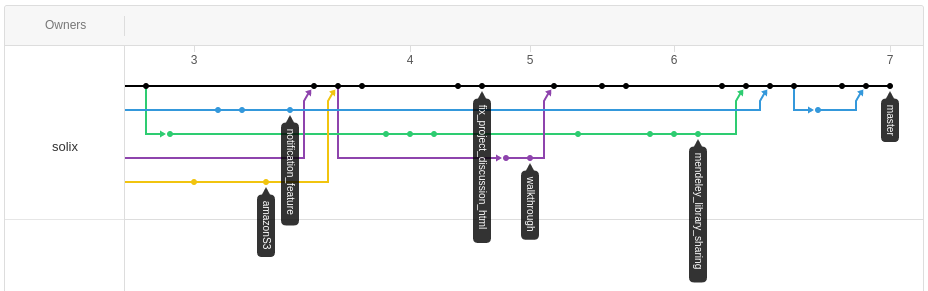
\includegraphics[scale=0.3]{./images/github_tree.png}
		\caption{GitHub Branching Tree}
	\end{figure}
\end{frame}

%METRICS 2
\begin{frame}
\frametitle{Metrics \& Evaluation}
\framesubtitle{Scrum}
	\begin{figure}
		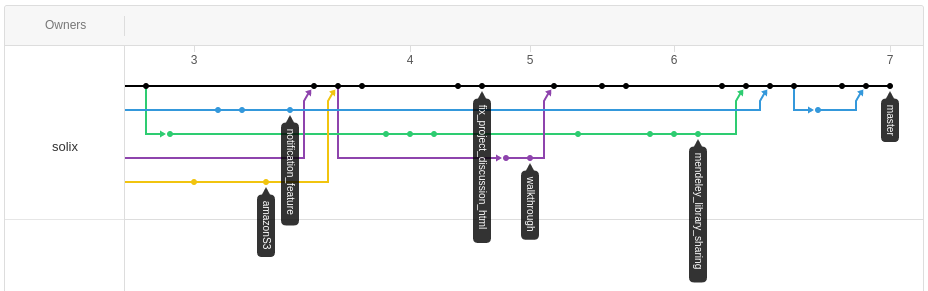
\includegraphics[scale=0.3]{./images/github_tree.png}
		\caption{GitHub Branching Tree}
	\end{figure}
\end{frame}

\end{document}
